
\newcommand{\nomedoc}{Manuale Utente}
\newcommand{\versione}{2.0}
\newcommand{\versioneglossario}{3.0}
\newcommand{\versionenormeprogetto}{3.0}
\newcommand{\nomefile}{ManualeUtente-\versione.pdf}
\newcommand{\datacreazione}{24 Febbraio 2011}
\newcommand{\datamodifica}{27 Febbraio 2011}
\newcommand{\stato}{formale}
\newcommand{\uso}{esterno}
\newcommand{\redazione}{Baron Federico}
\newcommand{\verifica}{Cosimo Caputo}
\newcommand{\approvazione}{Mandolo Andrea}
\newcommand{\distribuzione}{
VT.G \\
& Prof. Vardanega Tullio\\
& Prof. Cardin Riccardo }

% FUNZIONI TIPOGRAFICHE
\newcommand{\co}{\texttt} % courier
\newcommand{\bo}{\textbf} % bold
\newcommand{\pr}{\par\medskip} % paragrafo spaziato
\newcommand{\sca}{\textsc} % small caps

\documentclass[a4paper,12pt]{report}
% 10pt,11pt,12pt
% titlepage, notitlepage -> per dare inizio o no ad una nuova pagina dopo titolo
% twoside -> per dire se fronte-retro
\usepackage[latin1]{inputenc}
% per caratteri accentati
\usepackage[italian]{babel}
% per regole sintattiche italiane
\usepackage[bookmarks=true, pdfborder={0 0 0 0}]{hyperref}
% per collegamenti ipertestuali
\usepackage{graphicx}
% per inserimento immagini

% \usepackage{enumerate}
% per personalizzare elenchi puntati

\usepackage[hmargin=2cm]{geometry} %margine 2 cm
%\geometry{options varie}

% comandi per gestire meglio header e footer
\usepackage{fancyhdr}  % header e footer
\usepackage{totpages}
\pagestyle{fancy}
\renewcommand{\headrulewidth}{0.4pt}
\renewcommand{\footrulewidth}{0.4pt}

\setlength{\headheight}{1.2cm} % NON TOCCARE
\setlength{\voffset}{-1.5cm} % NON TOCCARE
\setlength{\textheight}{666pt} % NON TOCCARE
\setlength{\footskip}{60pt}
\setlength{\parindent}{0pt} % INDENTAZIONE

\lhead{\nomedoc\  (ver. \versione)}
\chead{}
\rhead{
\includegraphics[height=1cm]{img/netmus.png}}
\lfoot{
\includegraphics[height=0.8cm]{img/logo.png}}
\cfoot{}
\rfoot{\thepage}

\usepackage{titlesec}
\titleformat{\chapter}{\normalfont\huge\bfseries}
{\thechapter}{20pt}{\Huge}

\usepackage{rotating}   % PER TABELLE E AMBIENTI RUOTATI
\usepackage{array}
\usepackage{color}
\usepackage{colortbl}  % VARIE PER GESTIRE I COLORI
\definecolor{Orange}{RGB}{255,127,0}   % ARANCIO ACCES0
\definecolor{orange}{RGB}{255,207,80}  % ARANCIO TENUE

\addtocontents{toc}{\protect\thispagestyle{fancy}}  % PER INDICI CON + PAGINE
\usepackage[font=it]{caption}    % PER RENDERE CORSIVE LE DIDASCALIE
\usepackage{eurosym}  % PER SIMBOLO EURO

% \usepackage{listings}   per codice sorgente

\author{VT.G - Valter Texas Group}

\begin{document}

\pagenumbering{Roman} % INIZIO NUMERAZIONE ARABA

\vspace*{1cm}
\begin{center}

\begin{LARGE} \sca{Federico Baron} \end{LARGE}\\
\vspace{0.5cm}
\begin{Large}
\emph{fede.baron.89@gmail.com} \end{Large}\\
\vspace*{1cm} 
\includegraphics[width=5cm]{img/logo.png}\\
\vspace{0.5cm}
\begin{Large} \emph{``Comunicazione Aumentata/Alternativa per Giovani Ospiti
della Terapia Intensiva Pediatrica''} \end{Large}\\
\vspace{3cm}
\begin{Large} \sca{\nomedoc} \end{Large}\\
\end{center}
\vspace{1cm}

% INFORMAZIONI DOCUMENTO
\begin{center}
\begin{tabular}{r|l}
\hline & \\
\bo{Nome} & \nomefile \\
\bo{Versione attuale} & \versione \\
\bo{Data creazione} & \datacreazione \\
\bo{Data ultima modifica} & \datamodifica \\
\bo{Redazione} & \redazione \\
& \\\hline
\end{tabular}
\end{center}
\newpage

\chapter*{Sommario}
\thispagestyle{fancy}
Il presente documento fornisce una guida chiara e semplice per l'utilizzo del
sistema NetMus.\\
Comprende un glossario con i termini meno conosciuti e un'appendice con i
problemi pi\`u comuni, possibili cause e soluzioni proposte.

\newpage
% REGISTRO MODIFICHE
\section*{Registro delle modifiche}

\begin{longtable}{|p{0.13\textwidth}|c|p{0.2\textwidth}|p{0.46\textwidth}|}
\hline
\rowcolor{orange} \bo{Data} & \bo{Versione} & \bo{Autore} & \bo{Descrizione} \\
\hline
\endhead
\hline
\endfoot
14/03/2011 & 2.0 & Caputo Cosimo & Documento validato per consegna RA.\\
\hline
19/03/2011 & 1.4 & Daminato Simone & Verificato il documento.\\
\hline
19/03/2011 & 1.3 & Trezzi Giovanni & Aggiornati gli screenshots.\\
\hline
12/03/2011 & 1.2 & Lovato Daniele & Finito di redarre il documento.\\
\hline
5/03/2011 & 1.1 & Baron Federico & Inseriti i messaggi di errore.\\
\hline
28/02/2011 & 1.0 & Mandolo Andrea & Validazione per consegna RQ.\\
\hline
28/02/2011 & 0.9 & Cosimo Caputo & Verificato l'intero documento.\\
\hline
27/02/2011 & 0.8 & Baron Federico & Corretti errori e Sistemata impaginazione
immagini.\\
\hline 
27/02/2011 & 0.7 & Palazzin Alberto & Aggiornato glossario, corretti un p\`o di
errori.\\
\hline
27/02/2011 & 0.6 & Daminato Simone & Inseriti gli screenshot nel documento.\\
\hline
26/02/2011 & 0.5 & Caputo Cosimo & Inizio creazione glossario.\\
\hline
26/02/2011 & 0.4 & Palazzin Alberto & Aggiunte nuove azioni possibili nella sezione
"Istruzioni per l'uso".\\
\hline
25/02/2011 & 0.3 & Baron Federico & Stesa parte preliminare delle istruzioni per
l'uso.\\
\hline
24/02/2011 & 0.2 & Daminato Simone & Stesura preambolo.\\
\hline 
24/02/2011 & 0.1 & Mandolo Andrea & Stesura prima versione del Manuale Utente.\\

\end{longtable}

% INDICE
\tableofcontents

\chapter{Introduzione}
\thispagestyle{fancy} % serve perche' nelle pagine di inizio Chapter esca header e footer
\pagenumbering{arabic} % INIZIO NUMERAZIONE NORMALE
\rfoot{\thepage\ di \pageref{TotPages}}
Questo manuale \`e destinato agli utilizzatori di \co{NetMus}, e comprende una
descrizione del prodotto e le istruzioni per l'uso, oltre a due appendici
riportanti gli eventuali messaggi di errore e il glossario.\\

Tutti i termini presenti nel glossario a termine del documento sono sottolineati
alla prima occorrenza \underline{in questo modo}.

\section{Definizione dell'utente del prodotto}
\co{NetMus} pu\`o essere utilizzato da chiunque: sono richieste solo poche
nozioni di base, ovvero come navigare in internet utilizzando un
\underline{browser web}.

\section{Come leggere il manuale}
Questo manuale presenta il prodotto \co{NetMus} e descrive le sue funzionalit\`a
e l'approccio dell'utente al suo utilizzo. In particolare, verranno illustrate
le azioni che l'utente pu\`o effettuare con questo software e come risolvere, se
possibile, gli eventuali problemi riscontrabili durante il suo l'utilizzo.

\section{Come riportare problemi e malfunzionamenti}
Per segnalare problemi e malfunzionamenti \`e disponibile un servizio online a
questo indirizzo: \url{http://code.google.com/p/netmus/issues/list}.\\
\`E sufficiente cliccare in alto a sinistra su \emph{New issue} (figura
\ref{fig:issues}), e nel modulo (figura \ref{fig:newIssue}) compilare i campi
col titolo (2) e la descrizione del problema (3).
\begin{figure}[!htbp]
  \centering
  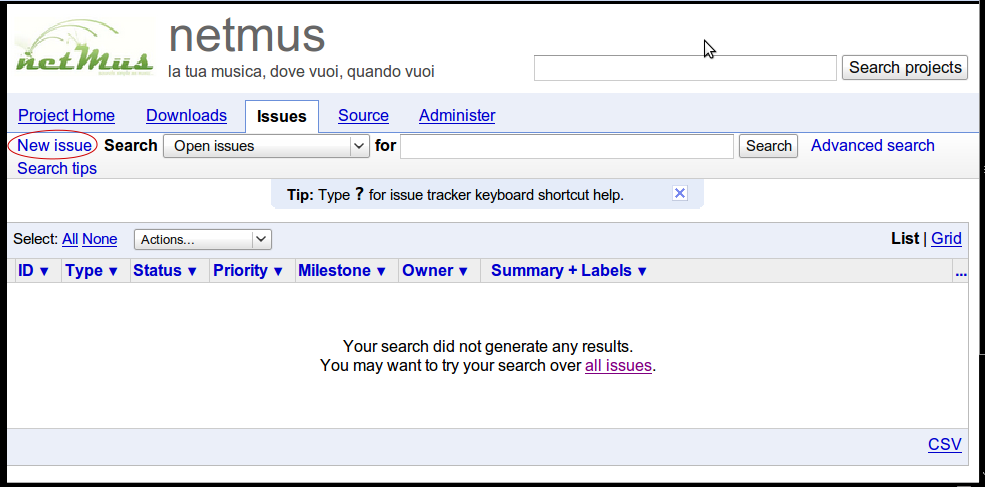
\includegraphics[width=16cm]{img/MU/issues.png}
\caption{Apertura di una nuova segnalazione}
\label{fig:issues}
\end{figure}

\begin{figure}[!htbp]
  \centering
  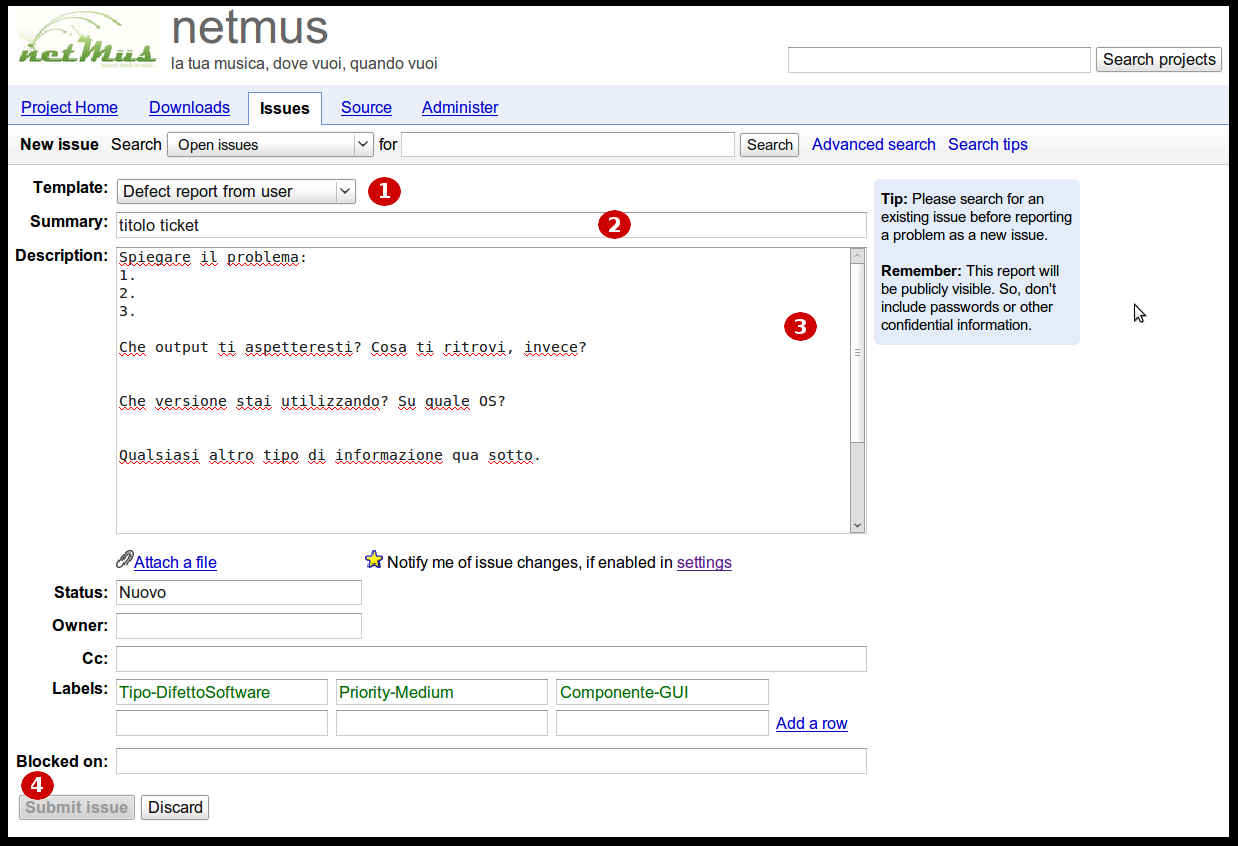
\includegraphics[width=16cm]{img/MU/new_issue.png}
\caption{Modulo per una nuova segnalazione}
\label{fig:newIssue}
\end{figure}

Come aiuto per descrivere il problema, consigliamo di selezionare il template
\emph{Defect report from user} (1), che contiene una traccia che aiuta ad
inserire tutte le informazioni necessarie.\\

Una volta compilato il modulo, premere il tasto ``Submit issue'' (4).

\section{Riferimenti informativi}
In case of further clarification on used technologies, or for further
help, you can refer to: \url{http://docs.google.com/support/
} .

\chapter{Descrizione generale}
\thispagestyle{fancy}
Oggigiorno, la maggior parte della musica che ascoltiamo \`e in formato digitale: \`e
per questo che nasce \co{NetMus}, uno strumento per gestire e condividere le
nostre canzoni preferite, che sfrutta le nuove tecnologie, come il
\underline{cloud computing}.\\

\co{NetMus} permette agli utenti di avere una
libreria virtuale online con tutte le canzoni che si ascoltano abitualmente, in modo da
poterle ascoltare ovunque ci si trovi.\\

Il prodotto \`e molto facile da utilizzare, una volta effettuato l'accesso
a \co{NetMus} basta collegare il proprio lettore mp3 e lasciarlo lavorare in
automatico, oppure indicargli in che cartella si tengono le canzoni: tutte le 
informazioni verranno estratte, analizzate, completate e
inserite nel nostro profilo, pronte per essere utilizzate.\\

Tra le possibilit\`a offerte, troviamo lo \underline{streaming} audio e video,
il completamento automatico delle informazioni dei brani, le playlist, e molto altro.\\

Il tutto \`e implementato con un'interfaccia grafica molto semplice che fornisce
tutte le funzionalit\`a necessarie, ma nonostante la sua semplicit\`a ha
un'impatto visivo notevole.

\chapter{Istruzioni per l'uso}
\thispagestyle{fancy}

\section{Descrizione funzionale}

Di seguito riportiamo una guida completa all'utilizzo di \co{NetMus}.\\
Verranno elencati dapprima i requisiti obbligatori per utilizzare il sistema,
successivamente verr\`a presentata una panoramica di \co{NetMus} dettagliata con
tutte le azioni che un utente pu\`o compiere per sfruttare le funzionalit\`a di
\co{NetMus}.

\subsection{Requisiti di Sistema per utilizzare NetMus}
\co{NetMus} \`e una web application che viene visualizzata attraverso il browser
web. Tuttavia non \`e sufficiente avere un browser web ed una connessione ad
internet per utilizzare questo sistema. 
\\
Qui di seguito presentiamo una chiara lista di
requisiti richiesti da \co{NetMus}.

\begin{itemize}
  \item Connessione ad Internet (superiore a 56k)
  \item Browser web (Google Chrome, Safari, Opera, Firefox*, IE**)
  \item La JVM (Java Virtual Machine) installata sul proprio PC
  \item Il plugin di Adobe Flash Player per la visualizzazione di video da
  Browser
  \item I JavaScript attivati sul proprio Browser
\end{itemize}

Anche solo senza uno di questi requisiti obbligatori,
non sar\`a possibile utilizzare alcune funzionalit\`a di \co{NetMus} o
addirittura tutto il sistema.\\
\\
\\

\emph{* Su Firefox le animazioni non vengono riprodotte, le funzionalit\`a del
sistema restano comunque completamente funzionanti}\\
\emph{** Per utilizzare NetMus su Microsoft Internet Explorer \`e
necessario scaricare il plugin Google Chrome Frame, poich\`e IE non supporta le
funzionalit\`a avanzate di NetMus: l'installazione verr\`a richiesta all'utente
alla prima apertura del programma}.

\newpage
\section{Utilizzare NetMus}
Vediamo qui di seguito come utilizzare \co{NetMus}.

\subsection{Registrazione}
Per iniziare ad utilizzare NetMus collegarsi all'indirizzo
\url{http://netmusbeta.appspot.com} . \\
\begin{figure}[!htbp]
  \centering
  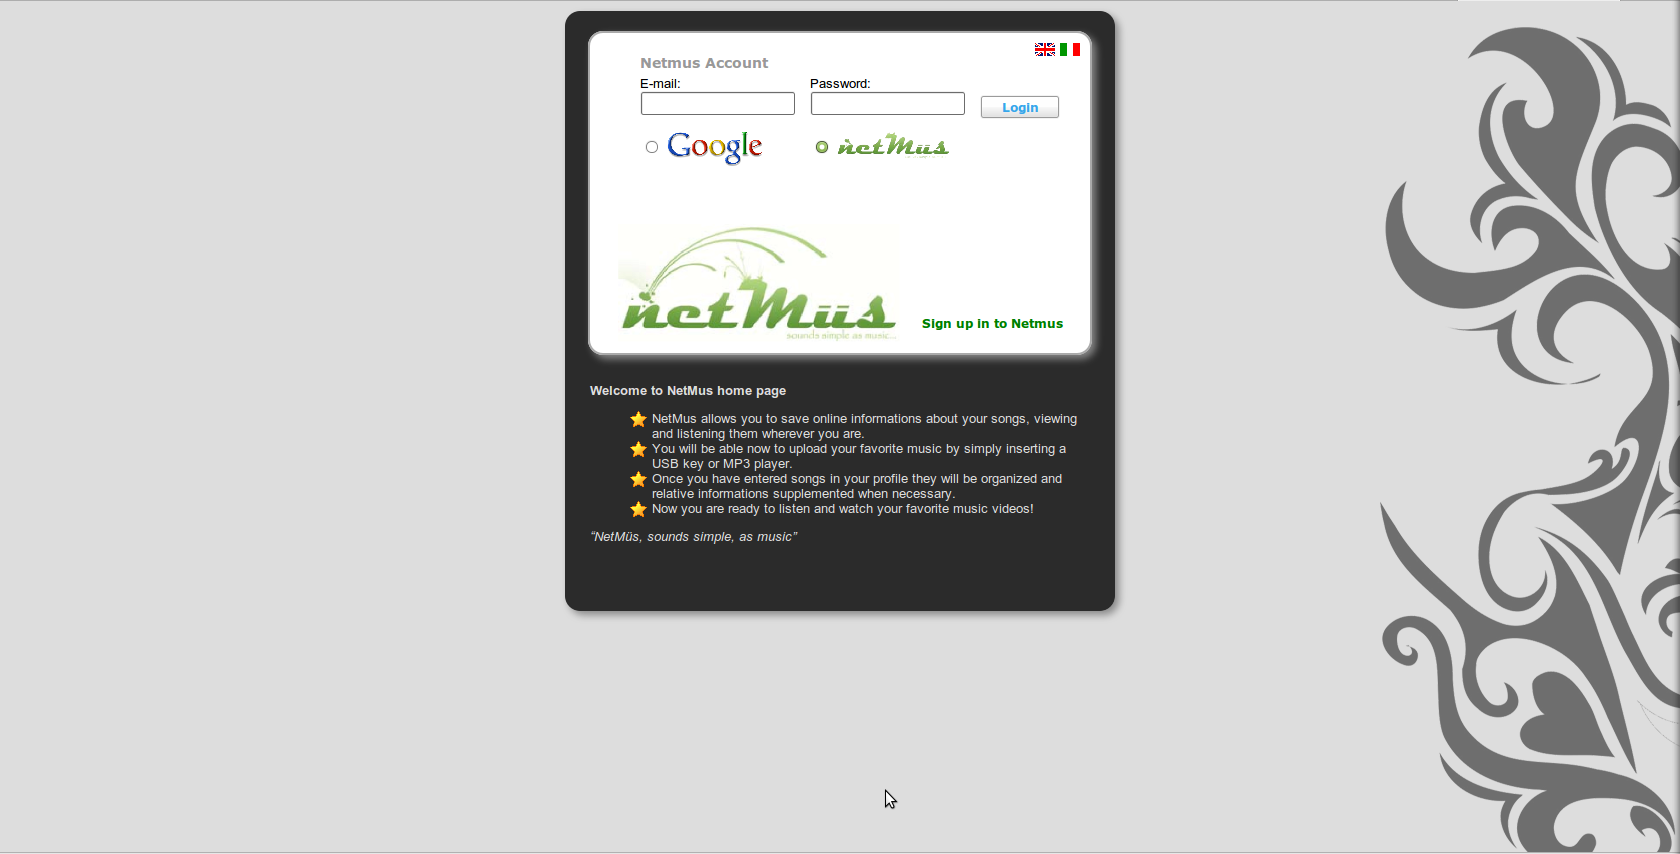
\includegraphics[width=14cm]{img/MU/login.png}
\caption{Interfaccia di NetMus Login}
\label{fig:login}
\end{figure}
\\
Qui vi verr\`a presentata la pagina di login (figura \ref{fig:login}) per
accedere al sistema. Se possedete gi\`a un account Google, potete effettuare
l'accesso direttamente con i dati dell'account di Google, dato che il sistema lo
permette, oppure registrarvi al sistema con un altro account.

\subsubsection*{Accesso tramite account Google}
Basta selezionare la scritta Google e cliccare sul tasto che ci appare ``Log in
NetMus using your Google Account'' (figura \ref{fig:loginGoogle}). Verrete
reindirizzati alla pagina di login di Google, dove potrete accedere con il
vostro account Google.

Una volta effettuato l'accesso, da Google verrete reindirizzati al sistema
\co{NetMus}, e potrete cominciare ad utilizzarlo.
\begin{figure}[!htbp]
  \centering
  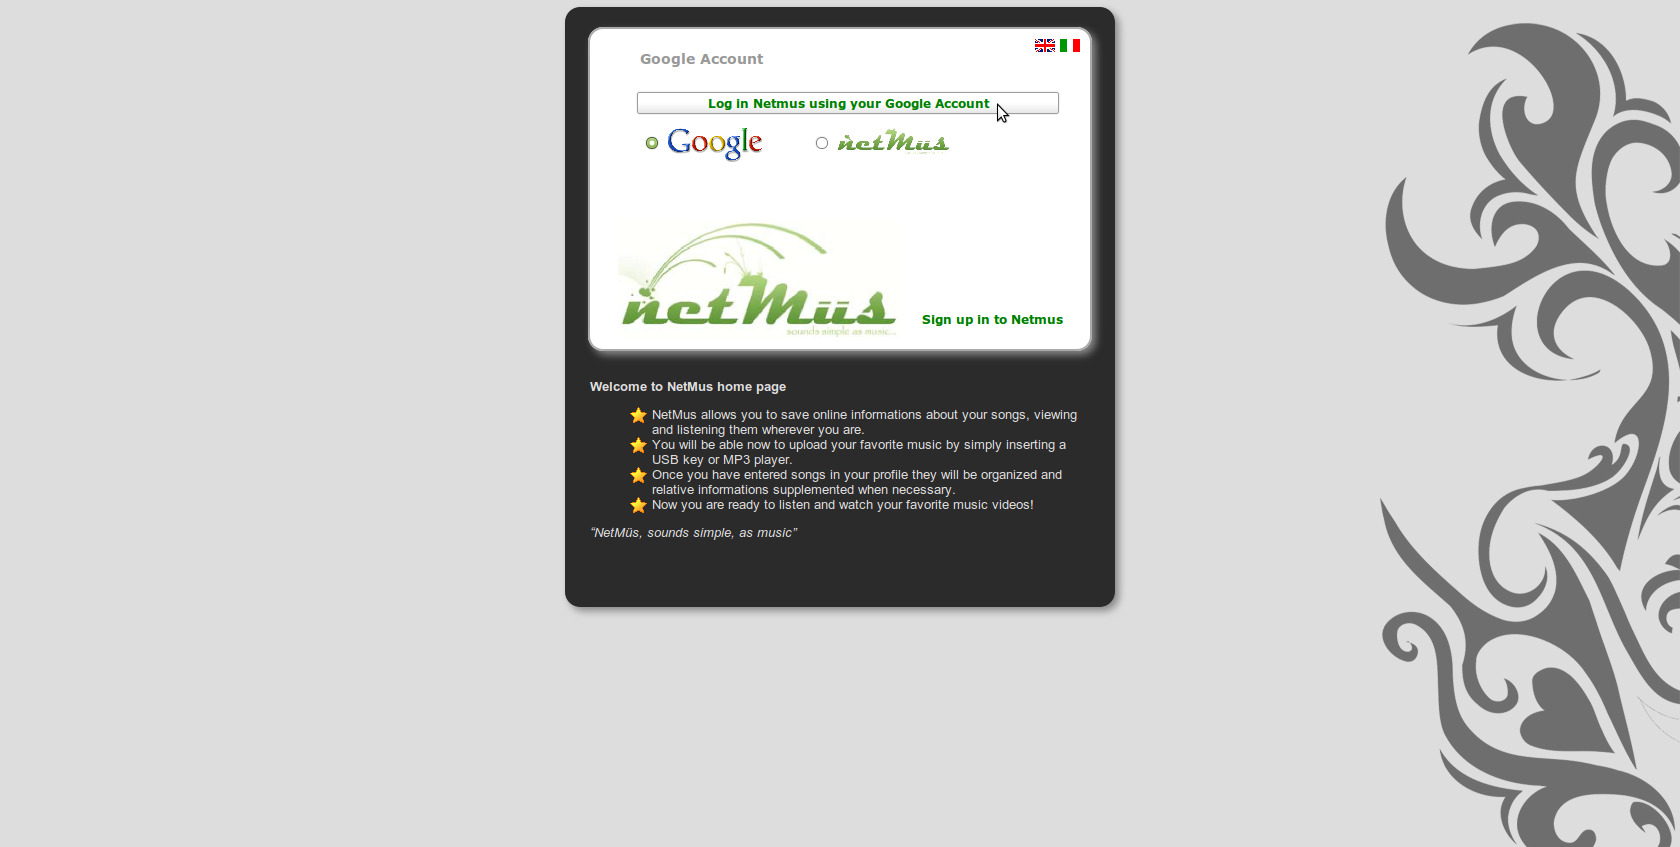
\includegraphics[width=14cm]{img/MU/loginGoogle.png}
\caption{Interfaccia per il Login Google}
\label{fig:loginGoogle}
\end{figure}

\subsubsection*{Creazione di un nuovo account NetMus}
Se invece non siete utenti Google oppure volete comunque crearvi un account
NetMus, al primo accesso \`e necessario che vi registriate al
sistema. La registrazione, cos\`i come l'utilizzo del sistema \co{NetMus},
\`e completamente gratuita.

Per accedere al modulo di registrazione basta cliccare alla voce ``Sign up in to
Netmus'', in basso a destra, e la view cambier\`a mostrandovi i campi per la
registrazione (figura \ref{fig:registrazione}).

\begin{figure}[!htbp]
  \centering
  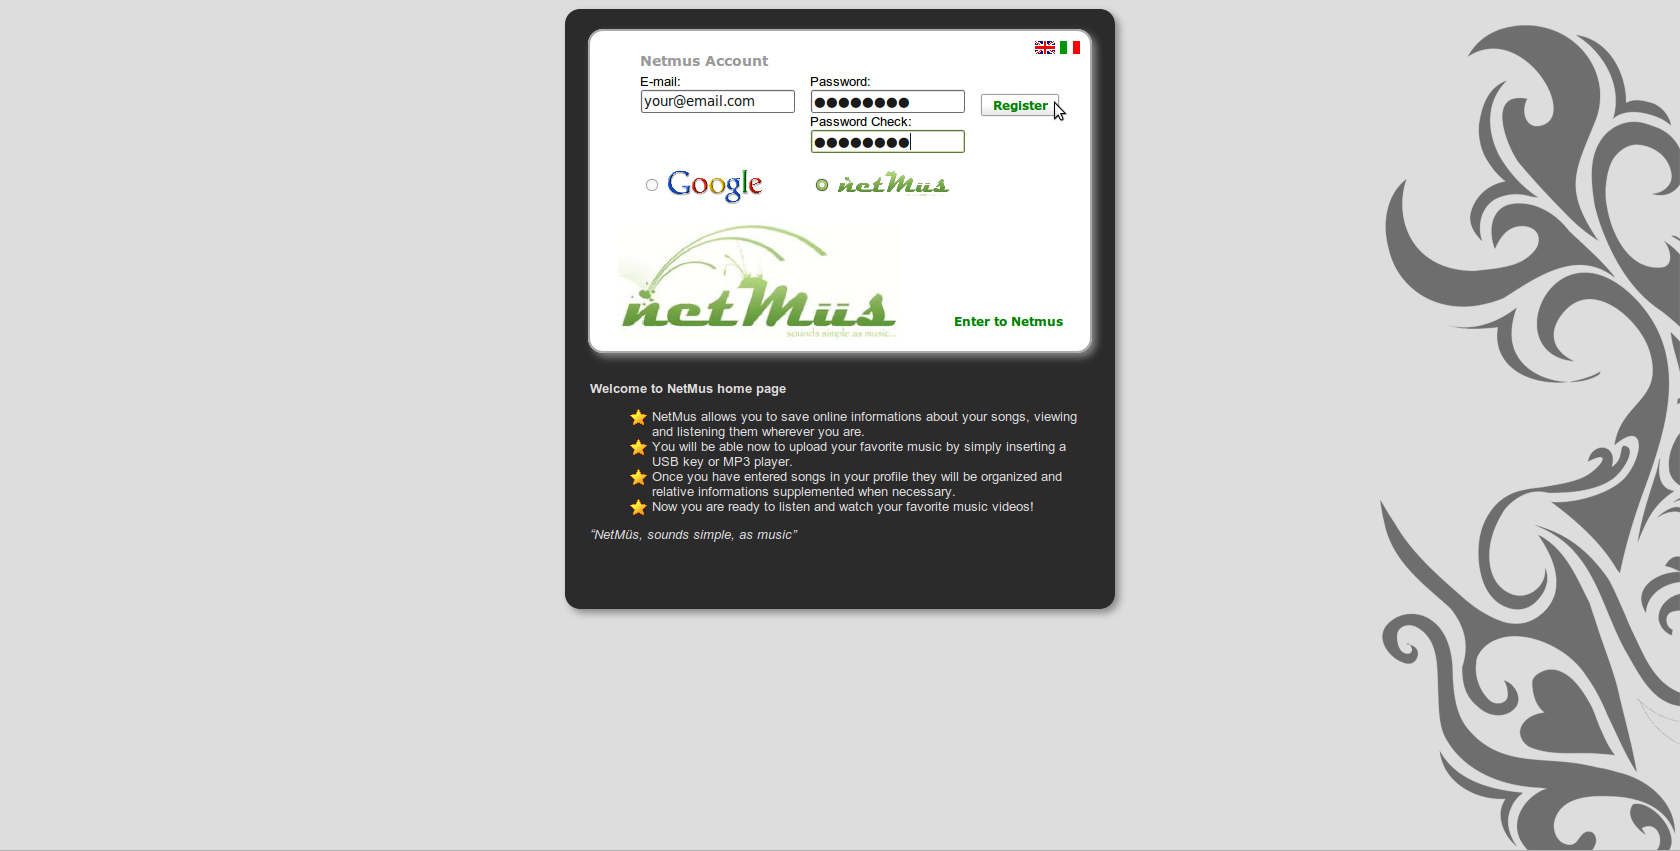
\includegraphics[width=14cm]{img/MU/registration.png}
\caption{Interfaccia di registrazione}
\label{fig:registrazione}
\end{figure}

La registrazione richiede un'email valida e una password composta da almeno 5
caratteri. Una volta creato il vostro account, avrete libero accesso al
sistema \co{NetMus}.\\

\newpage
\subsection{Primo accesso}

Al vostro primo accesso al sistema, durante il caricamento dell'interfaccia vi
verr\`a richiesto se eseguire l'applet firmata, dandogli il permesso di accedere
al vostro computer (figura \ref{fig:permessiApplet}).
\begin{figure}[!htbp]
  \centering
  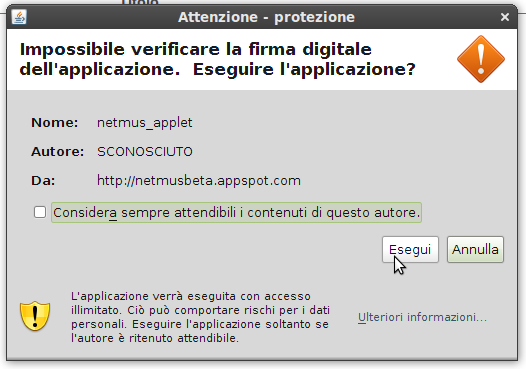
\includegraphics[width=10cm]{img/MU/permessi_applet.png}
\caption{Richiesta permesso di esecuzione dell'applet}
\label{fig:permessiApplet}
\end{figure}
L'applet in questione \`e il componente di \co{NetMus} che si occupa di cercare
gli mp3 nel vostro computer e di estrarne i dati: \emph{non raccoglie altre
informazioni sul vostro conto, e non contiene alcun virus}.

Se negate il permesso, l'applet non potr\`a accedere al contenuto del vostro
computer ed alle periferiche, impedendo quindi la raccolta delle informazioni
(non riuscirete quindi ad aggiungere dei brani).
Questa finestra di richiesta dell'autorizzazione verr\`a visualizzata ad ogni
accesso, a meno che non selezioniate ``Considera sempre attendibili i contenuti
di questo autore'' prima di cliccare su ``Esegui''.\\

L'interfaccia che vi verr\`a presentata sar\`a strutturata
in questo modo (figura \ref{fig:paginaPrincipale}):\\

\begin{figure}[!htbp]
  \centering
  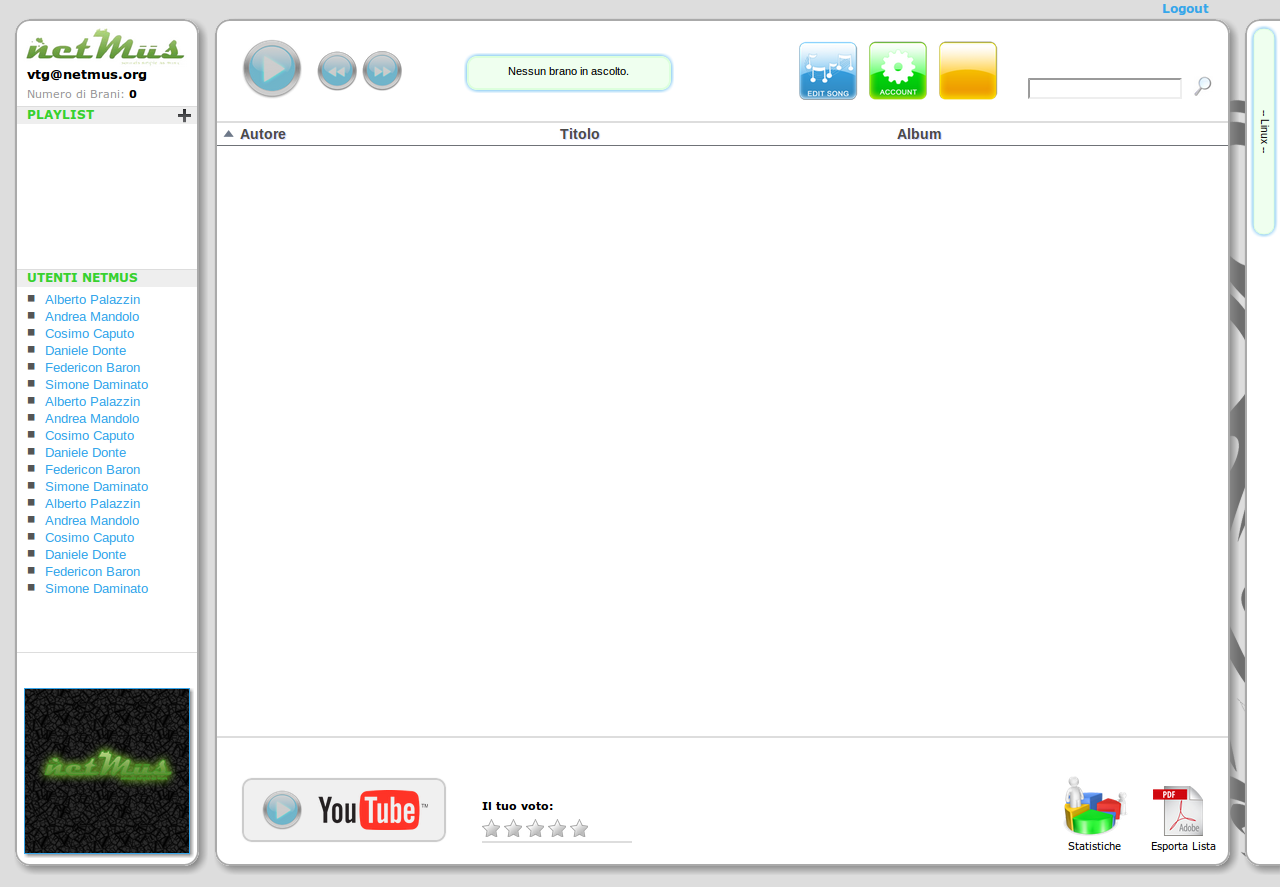
\includegraphics[width=14cm]{img/MU/profile_blank.png}
\caption{Pagina principale di NetMus al primo accesso}
\label{fig:paginaPrincipale}
\end{figure}

Ci sono tre parti principali: a sinistra troviamo la sezione delle
playlist (1), al centro quella dei brani (2), ed infine a destra c'\`e la
sezione dedicata all'applet(3).\\

Analizziamole in dettaglio (figura \ref{fig:appletbarAperta}):\\
\begin{figure}[!htbp]
  \centering
  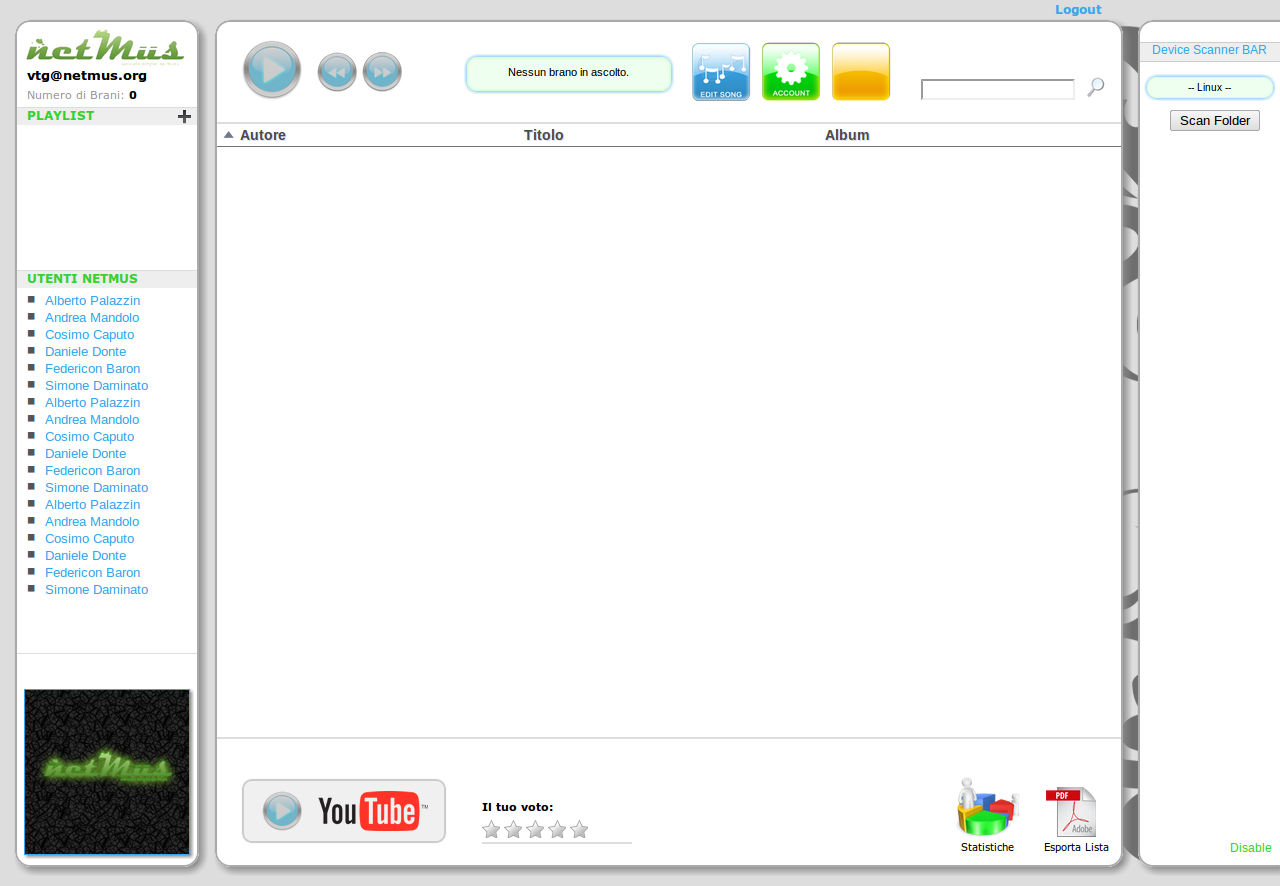
\includegraphics[width=14cm]{img/MU/applet_bar_open.png}
\caption{Pagina principale di NetMus con DEVICE SCANNER BAR espansa}
\label{fig:appletbarAperta}
\end{figure} 

Nel men\`u a sinistra, in alto (1) trovate il logo del sistema,
l'email con cui siete registrati (che viene utilizzato come vostro
\underline{nickname}), e il numero totale di brani presenti nel vostro catalogo,
che al momento sar\`a ovviamente pari a zero.\\
Subito sotto (2) si pu\`o vedere la lista delle playlist (al momento vuota
anche questa), dove verranno visualizzate tutte le vostre playlist create.\\

La sezione centrale dell'interfaccia \`e la pi\`u importante, \`e infatti il
nostro catalogo multimediale con player annessi e tasti per svariate azioni.\\
In particolare, in alto troviamo i pulsanti di controllo (3) e il form per la
ricerca di un brano (4) (vedere \ref{cap:ricerca}), poco pi\`u sotto (5) la
lista dei brani (al momento vuota), e in basso il player YouTube (6).\\

All'estrema sinistra della pagina \`e presente la barra per la scansione
dei \underline{dispositivi di archiviazione} \underline{di massa}(7), chiamata
pi\`u semplicemente ``DEVICE SCANNER BAR''.\\ 
Tale barra \`e visibile nella sua completezza solo al passaggio del mouse sopra
di essa: pu� comunque essere bloccata cliccando sul lucchetto presente
nell'angolo inferiore sinistro (8).\\
La barra permette la scansione manuale e visualizza l'avanzamento dell'analisi
ed estrazione automatica o manuale dei file mp3 da un dispositivo o da una \underline{directory} selezionata.\\
Inoltre, \`e possibile attivare o disattivare la scansione automatica cliccando
sulla scritta presente in basso a destra (9): quando \`e verde indica che la
scansione automatica \`e abilitata, quando \`e rossa invece indica che \`e
disattivata.

\newpage
\subsection{Iniziare ad utilizzare NetMus}

Per poter iniziare da subito a sfruttare la capacit\`a principale di \co{NetMus},
ossia quella di libreria musicale, \`e necessario caricare dei brani.
Per fare questo, si pu\`o inserire un dispositivo di archiviazione di massa
nella porta USB del proprio PC, o in alternativa \`e possibile scansionare
qualunque directory del proprio PC cliccando il tasto ``Scan Folder'' per la scansione manuale,
selezionare la cartella e premere ``OK'' (figura \ref{fig:scansioneManuale}).\\
\begin{figure}[!htbp]
  \centering
  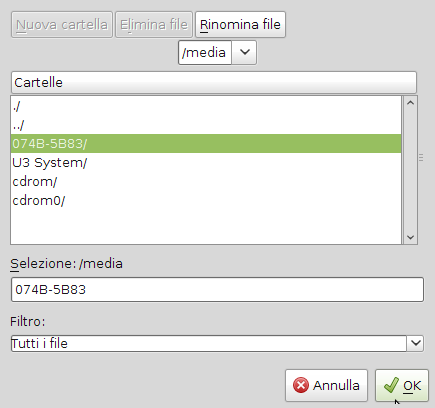
\includegraphics[width=14cm]{img/MU/scan_manual.png}
\caption{Interfaccia di selezione di una directory per la scansione
manuale}
\label{fig:scansioneManuale}
\end{figure}

Quando parte l'analisi, nella DEVICE SCANNER BAR viene visualizzato
l'avanzamento del processo, che mostra il numero di file analizzati fino al
messaggio ``Sending Done'' che indica che i file sono stati inviati alla
libreria musicale (figura \ref{fig:fineUpload}).
\begin{figure}[!htbp]
  \centering
  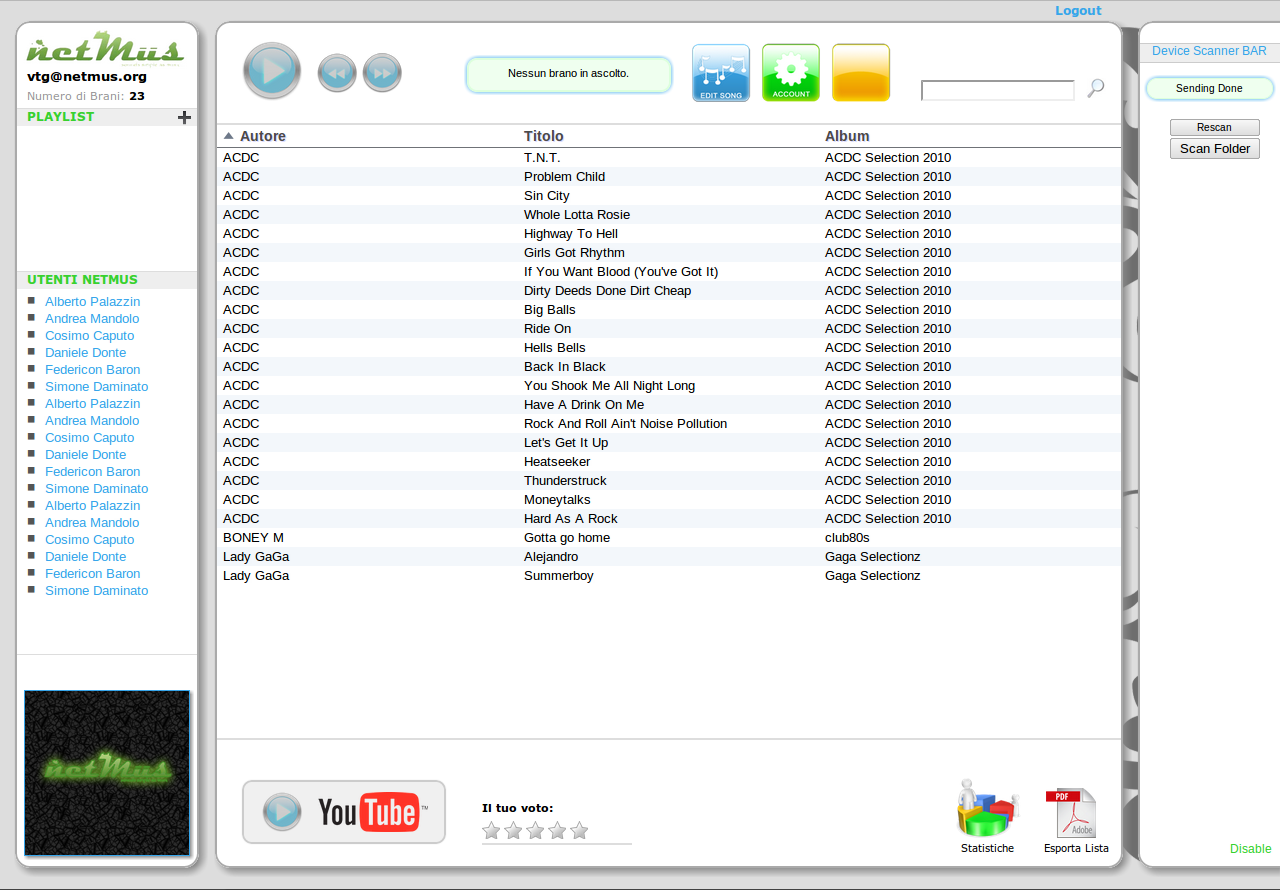
\includegraphics[width=14cm]{img/MU/song_loaded.png}
\caption{Interfaccia con catalogo multimediale caricato}
\label{fig:fineUpload}
\end{figure}

Una volta inviati, i brani compaiono sul catalogo multimediale.
A questo punto \`e possibile iniziare a sbizzarrirsi con le funzionalit\`a di
\co{NetMus}.\\

Le funzionalit\`a per comodit\`a di impostazione visiva e
sopratutto di ricerca, vengono elencate in sottoparagrafi.

\newpage
\section{Azioni richieste/permesse}
Di seguito presentiamo le azioni che \`e possibile eseguire sul sistema per
sfruttare le sue funzionalit\`a.

\subsection{Modalit\`a di visualizzazione del catalogo}
Il catalogo multimediale \`e la parte centrale del sistema \co{NetMus}. Qui
vengono elencati i brani raccolti dalla scansione dei vari dispositivi. E
possibile visualizzare il catalogo in due modalit\`a principali.\\
\\
La prima \`e la modalit\`a elenco (figura \ref{fig:fineUpload}). In questa
modalit\`a i brani vengono visualizzati come un elenco in cui sono visualizzati artista, titolo del brano e
album. In tale modalit\`a \`e possibile ordinare l'elenco dei brani per titolo,
artista o per album, semplicemente cliccando sulla barra superiore alle voci
``artista'', ``titolo'', ``album''.\\

La seconda modalit\`a di visualizzazione \`e quella in ``cover mode'' (figura
\ref{fig:coverMode}), ossia la visualizzazione dei brani con la copertina del
proprio album. Questa \`e una visualizzazione pi\`u carina da un punto di vista grafico ed estetico, ed \`e
pi\`u semplice riconoscere i brani che appartengono allo stesso album.\\

%da cambiare il nome dell'immagine!!! Sostituire con la nuova immagine corretta
\begin{figure}[!htbp]
  \centering
  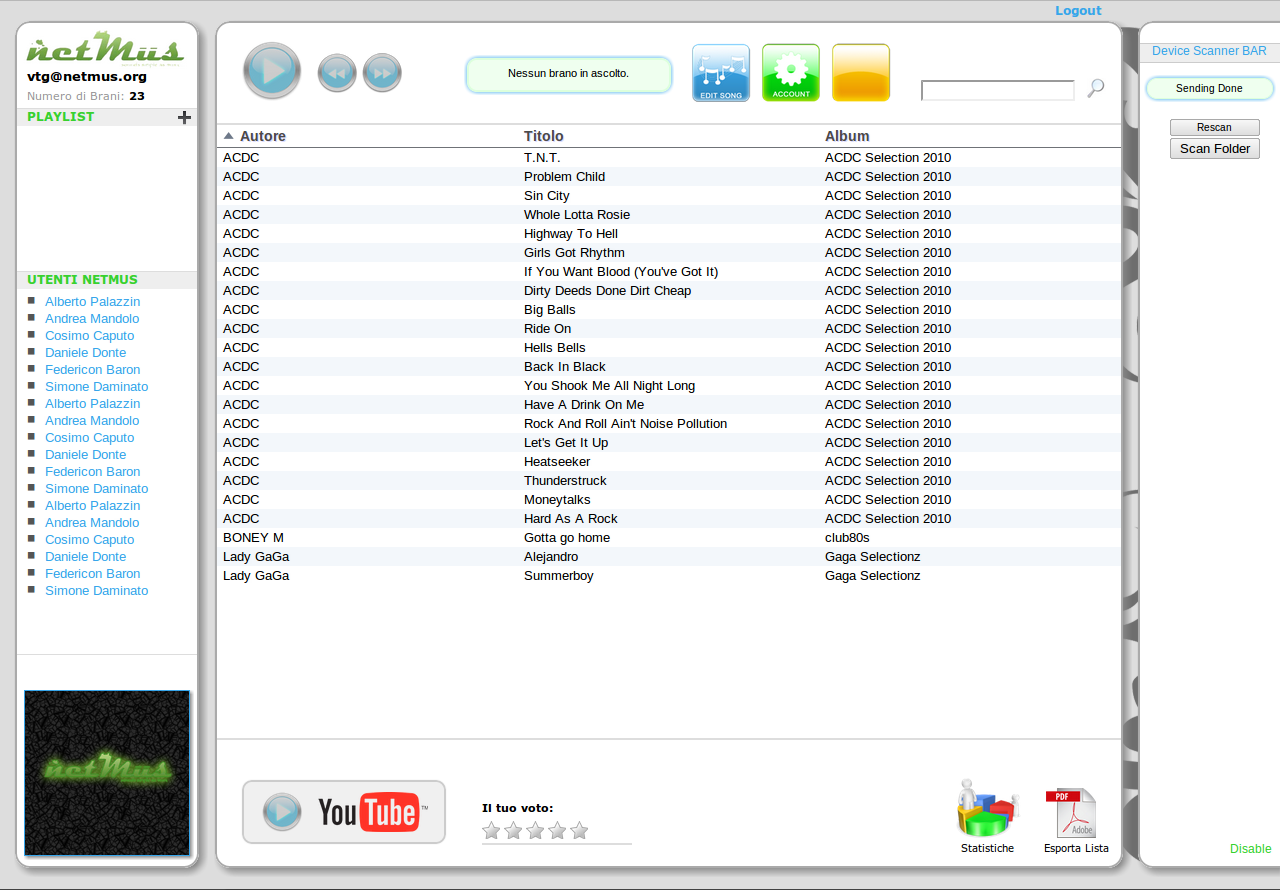
\includegraphics[width=14cm]{img/MU/song_loaded.png}
\caption{Interfaccia in ``cover mode''}
\label{fig:coverMode}
\end{figure}

\subsection{Ascoltare una canzone in streaming}

Passiamo ora alla descrizione della funzionalit\`a pi\`u
interessante del nostro prodotto, ossia la riproduzione delle tracce in streaming.\\
Per riprodurre una qualsiasi canzone del proprio catalogo, basta selezionarla e
quindi cliccare sul tasto play del \underline{player} in alto, o del player
YouTube in basso (figura \ref{fig:play}).\\ 
\begin{figure}[!htbp]
  \centering
  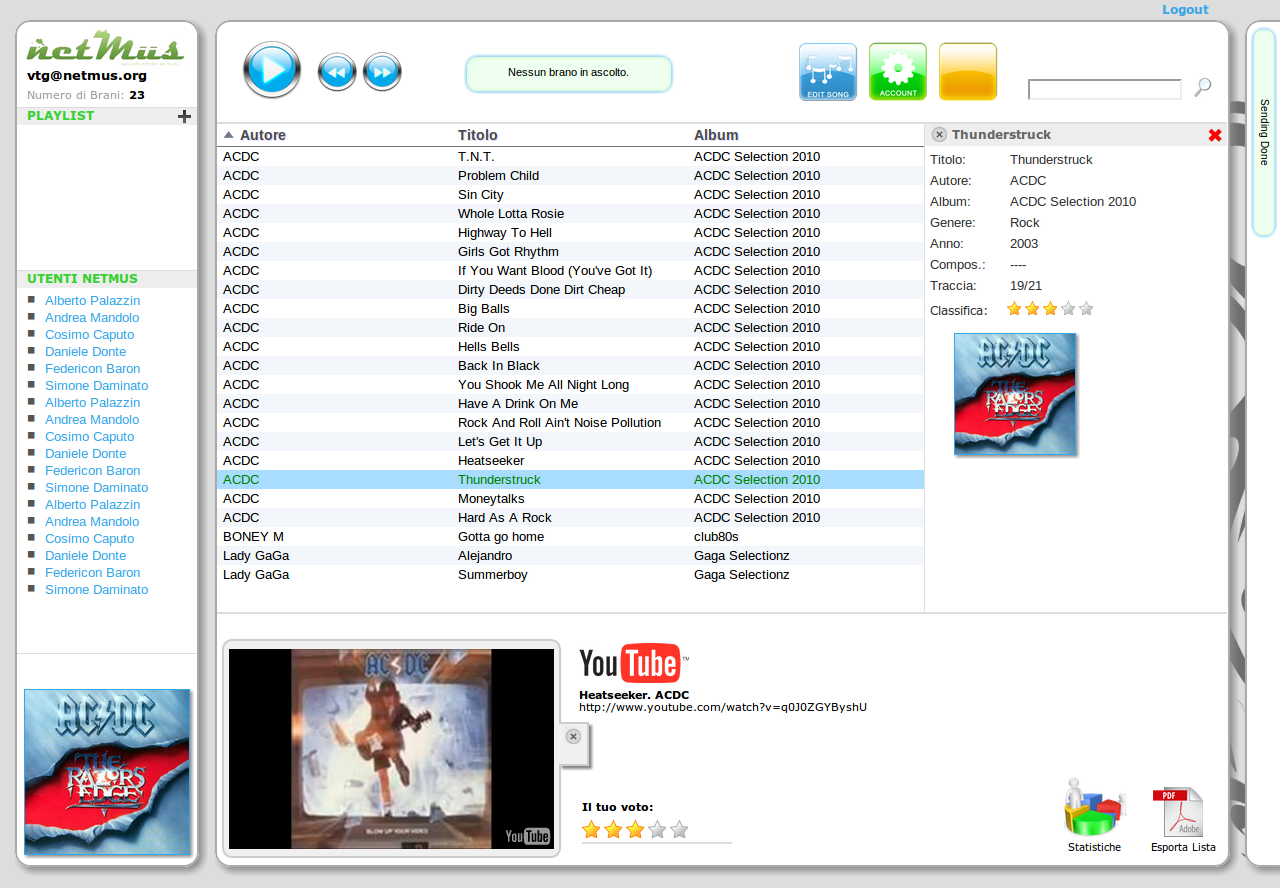
\includegraphics[width=14cm]{img/MU/player_youtube.png}
\caption{Interfaccia durante la riproduzione di un brano}
\label{fig:play}
\end{figure} 

Di fatto l'operazione svolta dai due player \`e la stessa, ma
si differenziano per il fatto che il player superiore (1) permette riproduzione
e pausa dello stream, passaggio al brano precedente e successivo del catalogo, mentre il player
inferiore si trasforma in un riproduttore di video in streaming, in cui viene
riprodotto il video musicale della canzone trovato da YouTube.
Inoltre tale player evidenzia il link di YouTube a cui \`e stato trovato il
brano, e con un click il browser ci reindirizza a tale link.\\
\`E possibile dare un voto alla canzone (2) da 1 a 5, cliccando sul numero di
stelle corrispondenti (vedere \ref{cap:voto}).\\

Per fermare la riproduzione di una canzone, potete mettere in pausa usando
l'apposito pulsante sul player in alto (1), oppure chiudere totalmente la
riproduzione premendo la ``x'' posta in alto a destra del video (3).\\

Al termine della riproduzione di un brano, il player passer\`a automaticamente a
riprodurre la successiva: se la lista era stata selezionata dal catalogo,
prender\`a la successiva da l\`i, se invece la canzone inizialmente era stata
selezionata da una playlist, verr\`a riprodotto il brano successivo di quella
playlist.

\subsection{Gestione playlist}

La creazione di una \underline{playlist} \`e un'operazione molto semplice e
comoda per poter avere una sequenza delle canzoni preferite.\\
Per creare una playlist (figura \ref{fig:playlist}) basta cliccare sul tasto
``+'' nel men\`u a sinistra di fianco alla voce ``PLAYLIST''(1). Subito comparir\`a un campo in cui
inserire il titolo della playlist: una volta inserito il titolo e premuto invio,
questa verr\`a creata e comparir\`a tra le playlist(2).\\
\begin{figure}[!htbp]
  \centering
  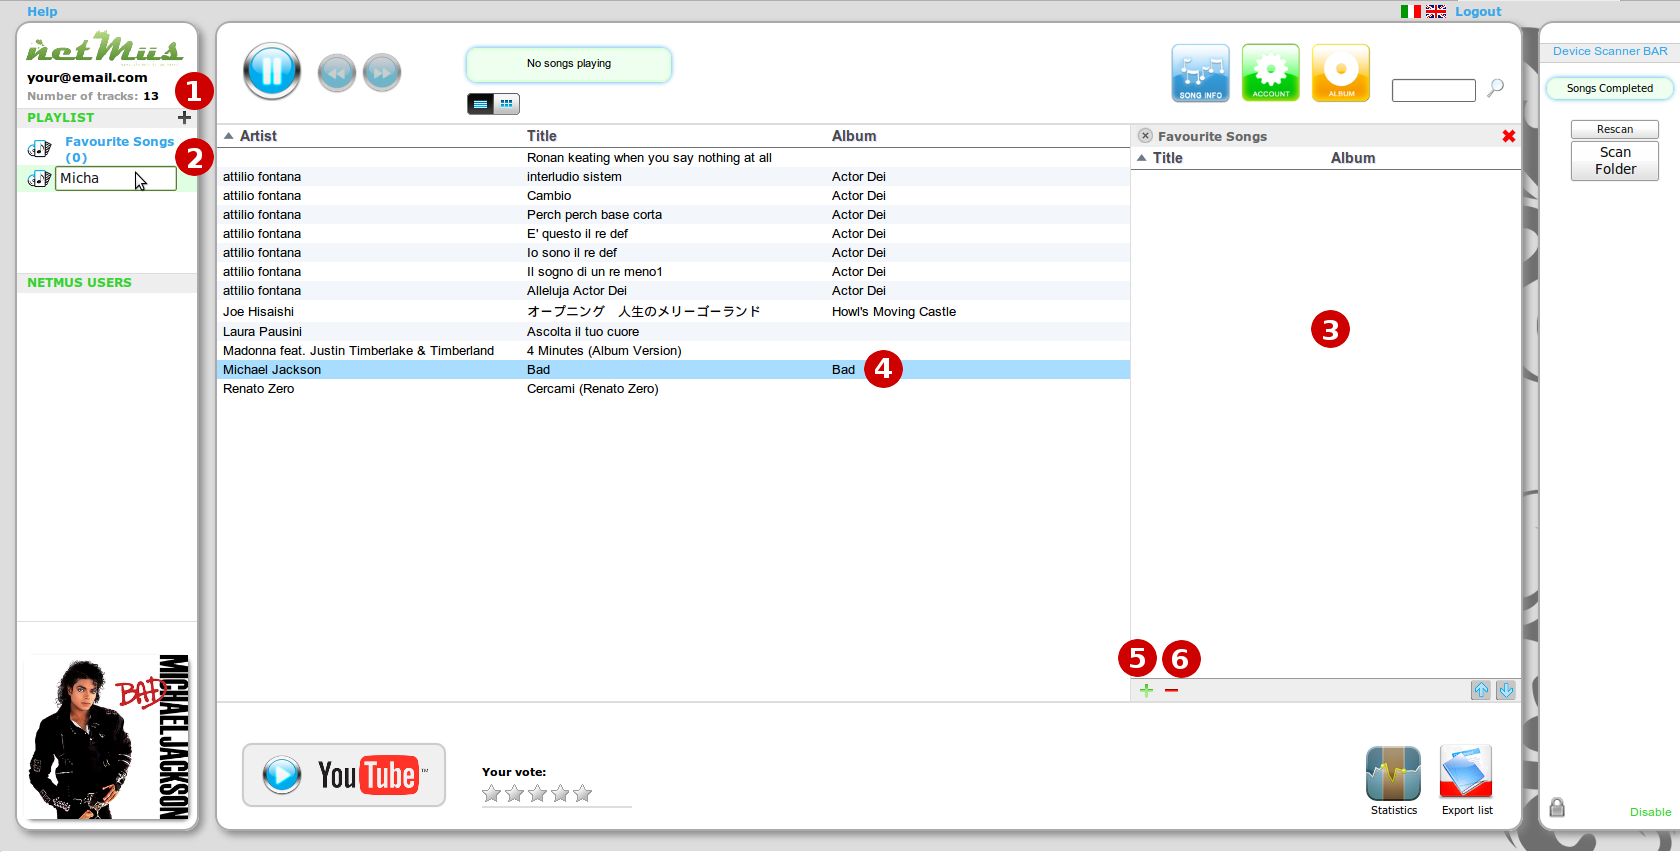
\includegraphics[width=14cm]{img/MU/new_playlist.png}
\caption{Pagina principale di NetMus durante la creazione di una playlist}
\label{fig:playlist}
\end{figure}
 
Ora non resta che inserire i brani all'interno della playlist
per ottenere la sequenza di canzoni desiderata. Per fare ci\`o basta cliccare sul
nome della playlist, si aprir\`a una finestra (3), vuota per il momento, in cui
andremo ad inserire i brani. Per inserire un brano basta
selezionarlo (4) e cliccarci due volte sopra, o alternativamente cliccare nella
finestra della playlist il simbolo ``+" verde (5).\\ 
La rimozione di un brano avviene in modo analogo; basta selezionare
nell'elenco dei brani della playlist il brano da rimuovere e successivamente
cliccare il simbolo ``-'' rosso (6), oppure premere sulla tastiera il tasto
``Del'' (in alcune tastiere chiamato anche ``Canc'').\\

Infine per eliminare una playlist basta selezionarla e cliccare la ``X'' rossa che
si trova nella finestrella in alto a destra (7).

\subsection{Visualizzare le informazioni riguardanti un brano}

Per visualizzare ulteriori informazioni riguardanti un brano (figura
\ref{fig:dettagli}) basta fare un doppio click sopra lo stesso. Si aprir\`a una
finestrella con l'elenco delle informazioni riguardanti il brano.\\
Notare che questa operazione non va effettuata con una playlist aperta,
altrimenti invece di visualizzare le informazioni del brano, quest'ultimo
verr\`a aggiunto alla playlist.\\

\begin{figure}[!htbp]
  \centering
  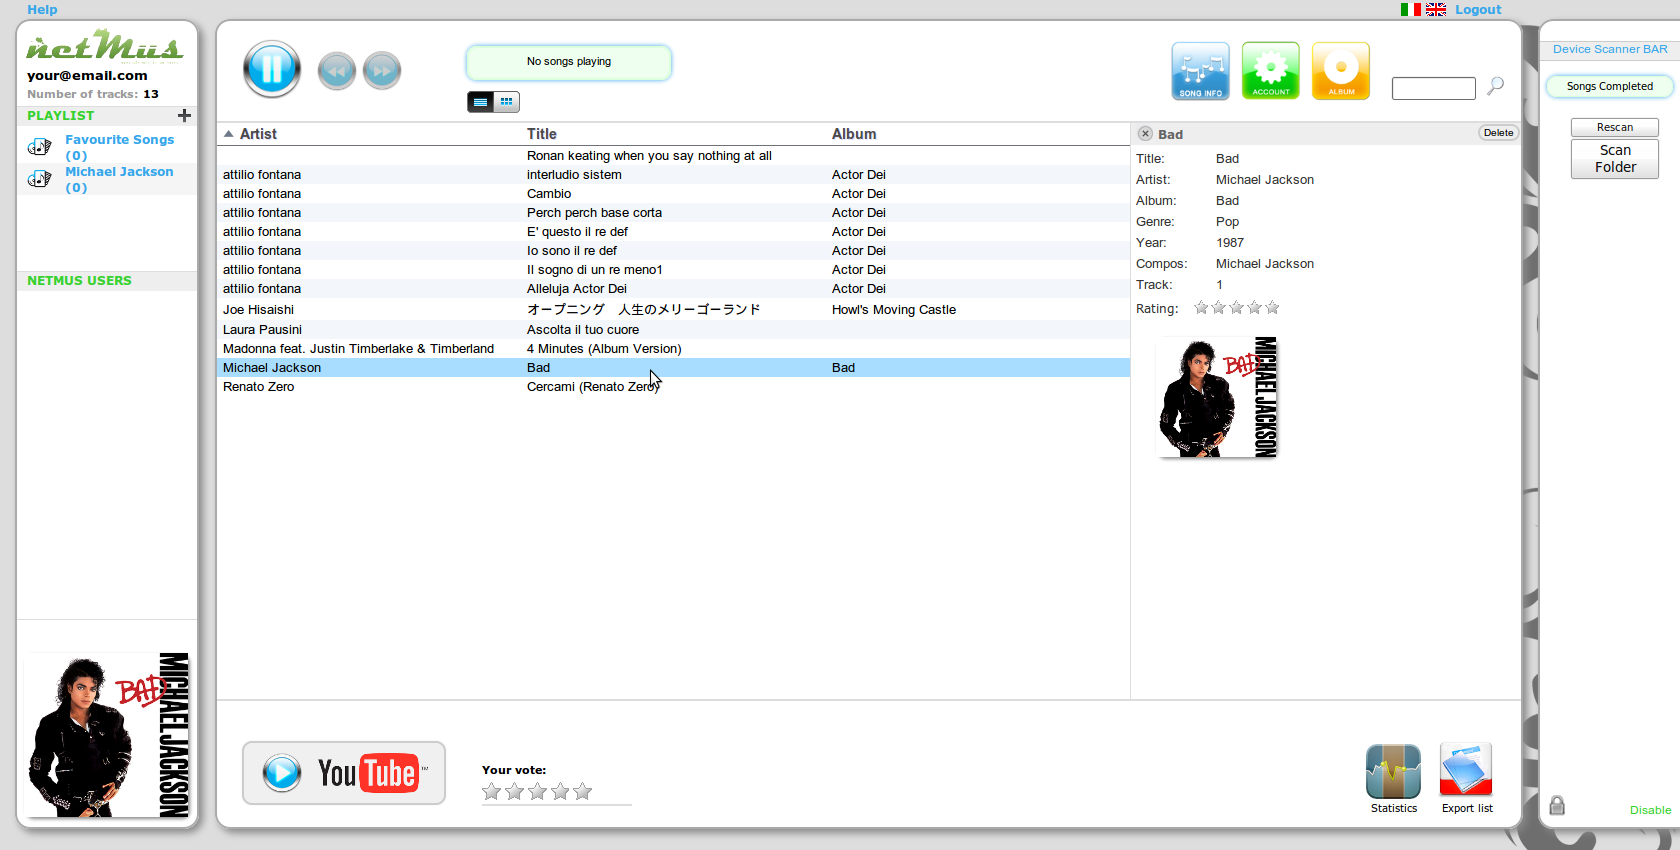
\includegraphics[width=14cm]{img/MU/info_song.png}
\caption{Dettagli di un brano del catalogo}
\label{fig:dettagli}
\end{figure}

Tra queste informazioni elenchiamo titolo, autore, album, genere, anno,
compositore, traccia, valutazione e copertina.\\
Per quanto riguarda la valutazione verr\`a spiegata pi\`u a fondo in seguito.\\
Le copertine invece vengono recuperate durante la memorizzazione del brano sul
catalogo.

\subsection{Eliminare un brano dal catalogo}

Per eliminare un brano dal proprio catalogo multimediale basta cliccarci sopra
due volte e fare apparire la finestrella con le informazioni dettagliate. A
questo punto cliccare il bottone rosso ``Elimina Brano'' come per le
playlist, e il brano verr\`a immediatamente eliminato dall'elenco.

\subsection{Ricercare un brano sul catalogo}
\label{cap:ricerca}
Per la ricerca di un brano all'interno del catalogo \`e stata implementata una
\underline{form} apposita (figura \ref{fig:appletbarAperta}, elemento 4). La
form, visualizzata nella pagina in alto a destra, ci permette di ricercare
titolo, album o artista di qualunque brano del catalogo.\\ 
La ricerca \`e immediata durante la digitazione, e i risultati vengono mostrati
direttamente sull'interfaccia principale del catalogo multimediale.

\subsection{Modificare le informazioni del profilo (anche cambio password)}

Nel sistema \co{NetMus} \`e possibile compilare ulteriori campi riguardanti il
proprio profilo utente.\\
Tale operazione \`e possibile cliccando sul tasto verde ``Account'', in alto a
destra.
Si aprir\`a un pop-up con l'elenco dei campi che \`e possibile
compilare (figura \ref{fig:profilo}): le informazioni dovranno essere inserite
in tali form.\\
\begin{figure}[!htbp]
  \centering
  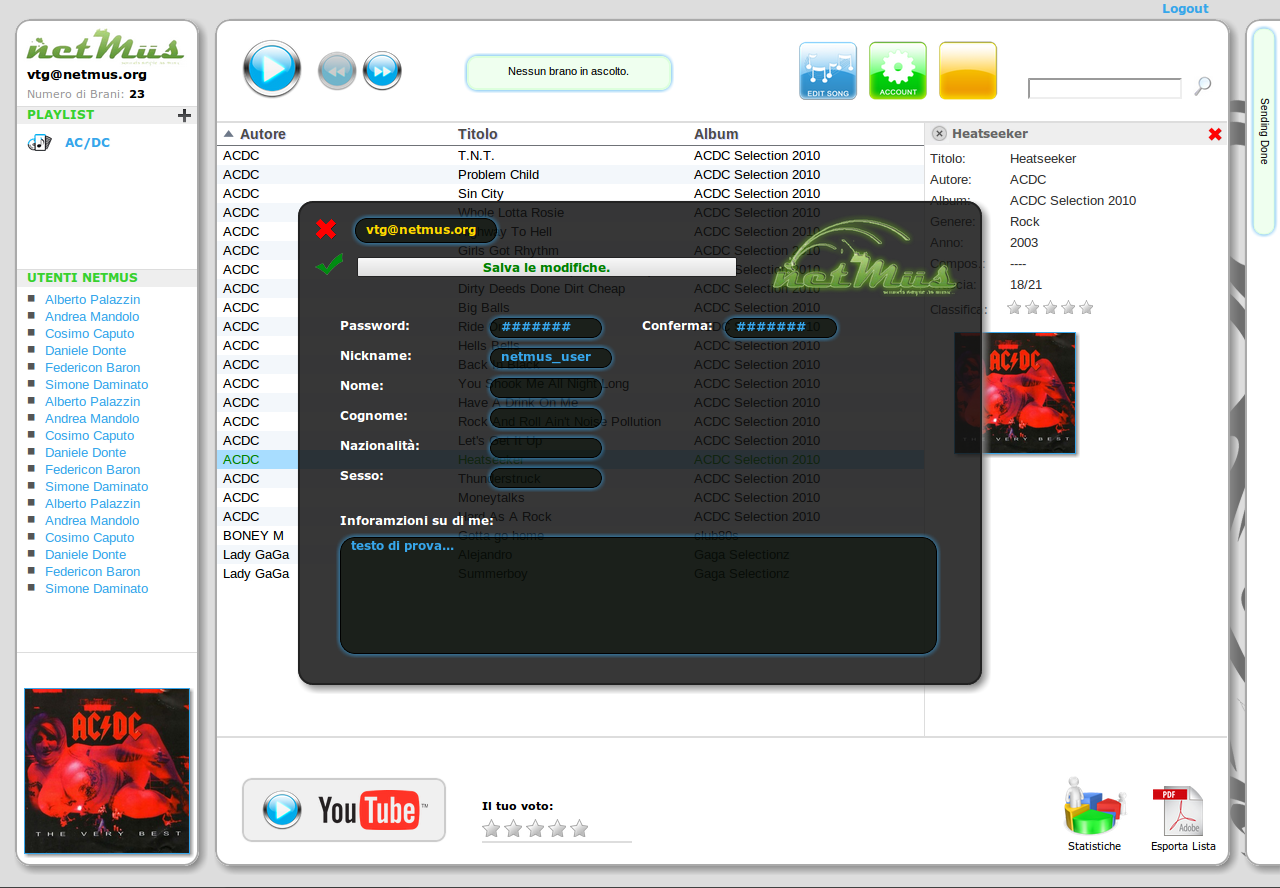
\includegraphics[width=14cm]{img/MU/profile_view.png}
\caption{Interfaccia per la modifica delle informazioni del profilo}
\label{fig:profilo}
\end{figure}

Le informazioni che \`e possibile aggiungere sono nickname, nome, cognome,
nazionalit\`a, sesso e una breve descrizione di s\`e. Da questa interfaccia \`e
anche possibile cambiare la propria password.\\

In particolare, per cambiare la password, bisogna inserire due volte la nuova
password che si intende utilizzare negli appositi campi (1).\\

Una volta inserite le nuove informazioni, cliccare su salva modifiche (2) per
salvare quanto editato, e cliccare sulla ``X'' grigia per chiudere la finestra
(3): se si chiude la finestra senza aver prima salvato le nuove informazioni,
queste verranno perse.\\

Per eliminare il proprio account invece, cliccare sulla ``X'' rossa (4): verr\`a
richiesta una conferma.

\subsection{Dare un voto ad un brano}
\label{cap:voto}
Il sistema \co{NetMus} offre anche la possibilit\`a di valutare un brano su una
scala da 1 a 5 stelline.\\
Da notare che il voto espresso per il brano, verr\`a poi visualizzato nelle
informazioni del brano ma sottoforma di media di tutti i voti ricevuti dai
possessori all'interno del sistema \co{NetMus} di quella stessa canzone.\\
Per valutare un brano basta selezionarlo dal catalogo con un click, e
successivamente cliccare sul numero di stelline desiderato in basso. Il voto
verr\`a automaticamente registrato tra le informazioni del brano in questione.

\subsection{Esportare il proprio catalogo multimediale in un documento Google}

Questa funzione originale \`e stata inserita per permettere l'esportazione del
catalogo multimediale in un documento Google, pi\`u adeguato alla stampa.\\
Per procedere con l'esportazione \`e necessario cliccare sul tasto in
basso a destra ``Esporta Lista''. A pressione avvenuta, il sistema
auto-generer\`a un documento con l'elenco dei brani del catalogo, e
visualizzer\`a risultato, dove l'utente potr\`a guardarlo, stamparlo e/o
salvarlo.

\subsection{Visualizzare le statistiche del sistema e del proprio account}

Per visualizzare le statistiche del proprio sistema basta cliccare sul tasto
``Statistiche'' in basso a destra. Verranno dunque visualizzate su un pop-up le
statistiche riguardanti il sistema \co{NetMus} (canzone pi\`u gettonata, numero
di utenti, ecc..) e le statistiche riguardanti il proprio account (canzone pi\`u
ascoltata, genere preferito, autore preferito, ecc..).

\section{Errori probabili e cause possibili}

\subsection*{Il dispositivo USB non viene analizzato}
\begin{itemize}
  \item controllare che la DEVICE SCANNER BAR non sia disabilitata. La DEVICE
  SCANNER BAR \`e disabilitata quando nell'angolo in basso vi \`e la scritta
  verde ``Enable''.
  \item se non era stato dato il permesso all'applet di essere eseguita, \`e
  normale che non funzioni. In questo caso, chiudete il browser web e
  riapritelo, tornando su \co{NetMus} vi verr\`a chiesto nuovamente il
  permesso.
\end{itemize}

\subsection*{Alcuni brani analizzati non sono stati caricati nel catalogo}
\begin{itemize}
  \item controllare che non fossero gi\`a stati analizzati e inseriti nel
  catalogo durante un' analisi precedente. Per essere sicuri, controllare il log
  presente all'interno del dispositivo in cui \co{NetMus} ha fatto la scansione.
  \item i brani non hanno i tag necessari completi. Se un brano non ha i
  tag artista titolo e album completi il brano non viene catalogato perch\`e non
  c'\`e modo di riconoscere quale brano sia.
  \item i tag sono presenti, ma corrotti. Pu\`o capitare che coi brani scaricati i tag
  siano presenti ma non leggibili. Provate a modificarli con un programma qualsiasi, e 
  a salvarli, molto probabilmente risolver\`a il problema.
\end{itemize}

\subsection*{La canzone riprodotta dal player di YouTube non \`e quella
corretta}
\begin{itemize}
  \item purtroppo la ricerca su YouTube non va sempre a buon fine: questa cosa
  non dipende dal nostro software.
  \item i tag delle canzone desiderata sono sbagliati e quindi la
  ricerca di tale canzone produce risultati errati. Modificare le informazioni
  della suddetta canzone per risolvere il problema.
\end{itemize}

\subsection*{La copertina dell'album non viene visualizzata}
\begin{itemize}
  \item evidentemente la copertina dell'album in questione non \`e stata
  trovata dal nostro servizio di ricerca nella rete. Questo \`e possibile se
  l'album non \`e un album molto diffuso, oppure se il tag album nelle
  informazioni delle canzoni \`e errato o mal scritto.
\end{itemize}

\appendix % inizio appendice
\chapter{Messaggi di errore e loro significato}
\thispagestyle{fancy}
Presentiamo qui i messaggi di errore che \`e possibile riscontrare durante
l'utilizzo di \co{NetMus}: per comodit\`a sono divisi in sezioni che
rappresentano il contesto in cui si possono presentare.
\section{Login/registrazione}
\begin{description}
	\item[Impossibile connettersi al database :] errore generico che
	indica un problema interno del software. Il software potrebbe essere in manutenzione,
	riprovare pi\`u tardi.
	\item[Errore: la password deve avere almeno 5 caratteri :] la password
	che si pu\`o utilizzare ha un'unica restrizione: deve essere composta di almeno 5
	caratteri, quindi dovete sceglierne una pi\`u lunga.
	\item [Errore: le password non coincidono :] per confermare la
	password scelta bisogna ripeterla nell'apposito campo, e questo errore compare
	quando le due password non coincidono, in genere indica un errore di
	digitazione.
	\item[Errore: e-mail non valida :] l'email inserita non \`e valida:
	un'email valida \`e formata in questa maniera: account@provider.dominio (ad
	esempio: andrea@yahoo.it).
\end{description}

\section{AppletBar - aggiunta nuovi brani}
\begin{description}
	\item [Errore XML :] errore generico che
	indica un grave problema nell'analisi degli mp3. Provate a ri-effettuare una
	scansione: se il problema persiste, vuol dire che ci sono uno o pi\`u brani che
	creano problemi, provate nel caso a far analizzare solo una parte per volta
	degli mp3.
	\item [Errore INVIO :] c\`e un problema di comunicazione con l'applet:
	provate a chiudere e riaprire il browser, tornando su \co{NetMus}. Se
	riscontrate ancora lo stesso messaggio di errore, aggiornate la Java Virtual
	Machine.
	\item [Errore invio brani: problema durante l'invio dei brani al server :] c\`e
	un problema di comunicazione col server, riavviate l'applicazione.
\end{description}

\section{Playlist}
\begin{description}
	\item [Errore: nuova playlist non creata :] indica che non \`e stato
	possibile creare la nuova playlist. Probabilmente ne esiste gi\`a una con lo
	stesso nome.
	\item [Errore: playlist non rimossa :] non \`e stato possibile
	eliminare la playlist: aggiornate la pagina.
	\item [Errore: canzone non aggiunta alla playlist :] c'\`e stato un
	problema nell'aggiungere la canzone alla playlist: aggiornate la pagina.
	\item [Errore: canzone non rimossa dalla playlist :] c'\`e stato un
	problema nella rimozione della canzone dalla playlist: aggiornate la pagina.
	\item [Errore: playlist non caricata :] c'\`e stato un errore durante
	il caricamento della playlist, probabilmente dovuto ad un errore di
	comunicazione col server. Riprovate a caricarla, ed eventualmente ad aggiornare
	la pagina: se il problema persiste, probabilmente \`e corrotta, quindi dovreste
	eliminarla e ricrearla.
	\item [Impossibile spostare la canzone :] c'\`e stato un errore nello
	spostare una canzone all'interno della playlist: ricaricatela e riprovate.
\end{description}

\section{Profilo}
\begin{description}
	\item[Errore: profilo non modificato :] c'\`e stato un errore nel salvare le
	ultime modifiche al profilo. Provate nuovamente.
	\item[Errore: utenti affini non caricati :] c'\`e stato un errore nel caricare
	gli utenti affini, tuttavia questo non compromette le funzionalit\`a del
	sistema: si pu\`o continuare ad usarlo normalmente, oppure aggiornare la
	pagina.
	\item[Errore: profilo utente non caricato :] grave errore durante il
	caricamento del profilo utente. Provate a riavviare il browser web.
	\item[Errore: Profilo utente non eliminato :] c'\`e stato un errore durante
	l'eliminazione dell'account. Riprovare in un secondo momento.
\end{description}

\section{Canzoni}
\begin{description}
	\item[Errore: canzone non eliminata :] c'\`e stato un errore durante
	l'eliminazione della canzone, ricaricate la pagina ed eventualmente riprovate.
	\item[Errore: informazioni canzone non caricate :] c'\`e stato un errore
	durante il recupero delle informazioni di una canzone: aggiornate la pagina.
	\item[Errore: voto non memorizzato :] non si \`e riusciti a salvare il voto per
	quella canzone: provate un'altra volta, ed eventualmente aggiornate la pagina.
	\item[Errore: statistiche non aggiornate :] le statistiche del sistema non sono
	aggiornate: si pu\`o comunque continuare ad utilizzare tranquillamente il
	sistema ed ignorare questo messaggio di errore.
	\item[Errore: documento non generato :] non \`e stato possibile generare il
	documento, molto probabilmente dovuto ai servizi esterni su cui si appoggia
	questa funzione: riprovate in un secondo momento.
	\item[Nessuna canzone votata :] indica semplicemente che l'utente non ha ancora
	espresso un voto su nessuna canzone.
	\item[Nessuna canzone possiede punteggio :] non \`e stato espresso alcun
	voto sulle canzoni, quindi non esistono canzoni pi\`u popolari rispetto ad
	altre.
\end{description}

\chapter{Glossario}
\thispagestyle{fancy}

\subsection*{Browser web:} programma che consente all'utente di navigare in
Internet. 'Netscape' e 'Internet Explorer' sono dei browser. 
\subsection*{Cloud computing:} un insieme di tecnologie informatiche che
permettono l'utilizzo di risorse o software distribuite in remoto.
\subsection*{Directory:} cartella (del computer).
\subsection*{Dispositivi di archiviazione di massa:} hard disk esterni, penne
usb, lettori mp3, eccetera.
\subsection*{Form:} parte di un'interfaccia grafica, in genere uno o pi\`u campi
dove vanno inseriti dei dati. 
\subsection*{Nickname:} nome utente.
\subsection*{Player:} riproduttore multimediale.
\subsection*{Playlist:} \`e una lista di canzoni, utilizzata su
personal computer e media player portatili per la gestione pi\`u rapida dei
brani in esecuzione e la loro sequenza.
\subsection*{Streaming:} un flusso di dati audio/video trasmessi da una sorgente
a una o pi\`u destinazioni tramite una rete telematica. Questi dati vengono
riprodotti man mano che arrivano a destinazione.

\end{document}
